\section{Esquema conceitual e paridade}\label{ap:signos}
Neste esquema, E designa signo estático, D dinâmico e M metalinguístico. O tipo de origem indica domínio, aplicação, transformação ou convenção. A condição de exposição vale igualmente para a projeção textual, antes de M1.

\begin{center}\small
\begin{tabularx}{\columnwidth}{@{}P{.22\columnwidth}YY@{}}\toprule
Signo/origem & Conteúdo e restrição & Expressão, observação e evento\\\midrule
Ocorrência (domínio) & Item alfabético fictício, data e hora & Cabeçalho ou opção com o mesmo texto (E/D). Evento: tela/ação\\
Data (domínio) & Hoje ou ontem; Hoje inicial & Opções de data e data ativa (E/D). Evento: ação/tela\\
Lembrete (aplicação) & Apresentado ou não; distinto do relato & Texto em detalhe quando visível (D). Evento: tela\\
Relato (aplicação) & Pendente inicial ou vigente, hora visível & Pendente / Sem confirmação registrada; Tomada relatada (D). Evento: tela/registro\\
Confirmação (aplicação) & A: breve; B: persistente & Salvo ou Tomada relatada com hora (D). Evento: ação/tela\\
Auditoria (aplicação) & Correção anterior; lista vazia por padrão & Relato anterior desfeito e hora (D). Evento: tela/correção\\
Histórico\newline (convenção) & Abrir lista por dia & Hist. ou Ver histórico (E). Evento: ação/tela\\
Último\newline transformado & Relato vigente mais recente, se houver & Último ou Ver último registro (E/D). Evento: ação/tela\\
Correção (aplicação) & Só relato vigente; exige confirmação & Lápis ou Corrigir relato; alerta e opções Confirmar/Cancelar (E/D). Evento: ação/correção\\
Relatar (aplicação) & Criar relato para item sem relato vigente & OK ou Registrar que tomei (E). Evento: ação/registro\\
Classificação (aplicação) & Domínio de respostas da tarefa; vazio inicialmente & Opções públicas; seleção exibida (E/D). Evento: ação/tela\\
Ajuda (aplicação) & Cartão e explicação expandida; sob pedido & Ajuda e texto compartilhado (M). Evento: pedido/entrega\\
Encerramento\newline (convenção) & Ações de encerrar & Controle explícito; tela de fim (E/D). Evento: fechamento\\\bottomrule
\end{tabularx}
\end{center}

Cabeçalhos, títulos e ações gerais aparecem em linguagem pública. Em R, a confirmação em A se perde após a próxima ação; a informação continua acessível em U/D. Nenhum signo carrega o identificador interno, o vetor de estados ou a correção esperada.

\section{CTT e referência analítica}\label{ap:ctt}
A: abstrata (raiz e grupos); U: operação mental / usuário; I: interação; S: processamento ou feedback do sistema. Usa-se $\gg$ para habilitar, $[\ ]\gg$ para habilitar com informação, $[\ ]$ para escolha e $|=|$ para ordem independente. $|>$ suspende, executa ajuda e retoma a origem; $[>$ desativa por desistência, teto ou falha. O processamento ocorre após a ação, sem inferência de leitura.

\begin{center}\small
\begin{tabularx}{\columnwidth}{@{}lY@{}}\toprule
Raiz abstrata & Grupos temporais\\\midrule
C2 & (Obter Alfa $|=|$ Obter Beta) $[\ ]\gg$ Comparar/responder $\gg$ Encerrar.\\
C4 & Pedir ajuda $\gg$ Conferir Gama $[\ ]\gg$ Classificar $\gg$ Encerrar.\\
V5 & Relatar horário $\gg$ (Conferir 18 h $|=|$ Conferir 08 h) $\gg$ Encerrar.\\
V8 & (Obter ajuda $|=|$ Consultar Gama $|=|$ Consultar Delta) $[\ ]\gg$ Classificar $\gg$ Encerrar.\\\bottomrule
\end{tabularx}
\end{center}

Em todas as raízes, envolver a tarefa com \textit{Tarefa $|>$ Consultar ajuda} no percurso opcional e \textit{Tarefa $[>$ Interromper}. Para C4/V8, a ajuda exigida é um grupo do percurso. A solicitação obrigatória não elimina outros pedidos. Não são usados operadores de paralelismo onde a interface exige uma ação de cada vez.


\noindent\begin{minipage}[t]{\columnwidth}
\footnotesize
\begin{tabularx}{\columnwidth}{@{}lYP{.15\columnwidth}@{}}\toprule
Folha & Ação herdada da HTA & Tipo\\\midrule
C2.1.1 & Abrir H em Hoje & I $\gg$ S\\
C2.1.2 & Abrir D de Alfa 08 & I $\gg$ S\\
C2.1.3 & Ler identificação e estado & U\\
C2.2.1 & Voltar ou abrir H; ou ir a U & I $\gg$ S\\
C2.2.2 & Abrir D de Beta 20 ou manter U coincidente & I $\gg$ S\\
C2.2.3 & Ler identificação e estado & U\\
C2.3.1 & Comparar e ordenar Alfa/Beta & U\\
C2.3.2 & Selecionar o par & I\\
C2.3.3 & Concluir & I $\gg$ S\\
C4.1.1 & Pedir ajuda; aguardar entrega & I $\gg$ S\\
C4.1.2 & Ler definições & U\\
C4.1.3 & Fechar cartão & I $\gg$ S\\
C4.2.1 & Manter R de Gama ou abrir H & I $\gg$ S\\
C4.2.2 & Abrir D de Gama & I $\gg$ S\\
C4.2.3 & Ler estado e aviso & U\\
C4.3.1 & Distinguir relato de ingestão & U\\
C4.3.2 & Selecionar classificação & I\\
C4.3.3 & Concluir & I $\gg$ S\\
V5.1.1 & Ler itens e horários; escolher alvo & U\\
V5.1.2 & Abrir R de Delta 18 & I $\gg$ S\\
\bottomrule\end{tabularx}
\end{minipage}
\newpage
\noindent\begin{minipage}[t]{\columnwidth}
\footnotesize
\begin{tabularx}{\columnwidth}{@{}lYP{.15\columnwidth}@{}}\toprule
Folha & Ação herdada da HTA & Tipo\\\midrule
V5.1.3 & Relatar uma vez & I\\
V5.2.1 & Abrir U & I $\gg$ S\\
V5.2.2 & Ler cabeçalho e conferir identidade & U\\
V5.2.3 & Ler estado após transação & U\\
V5.3.1 & Abrir H em Hoje ou U coincidente & I $\gg$ S\\
V5.3.2 & Abrir D de Delta 08 & I $\gg$ S\\
V5.3.3 & Ler estado e comparar horários & U\\
V5.4.1 & Concluir & I $\gg$ S\\
V8.1.1 & Abrir J e aguardar entrega & I $\gg$ S\\
V8.1.2 & Ler definições & U\\
V8.1.3 & Fechar cartão & I $\gg$ S\\
V8.2.1 & Abrir H ou voltar a H se preciso & I $\gg$ S\\
V8.2.2 & Abrir D de Gama 12 & I $\gg$ S\\
V8.2.3 & Ler estado e auditoria & U\\
V8.2.4 & Voltar a H se for abrir D & I $\gg$ S\\
V8.2.5 & Abrir D/U de Delta 18 & I $\gg$ S\\
V8.2.6 & Ler estado & U\\
V8.3.1 & Distinguir relato desfeito de válido e ingestão & U\\
V8.3.2 & Selecionar classificação de Gama & I\\
V8.3.3 & Concluir & I $\gg$ S\\
\bottomrule\end{tabularx}
\end{minipage}
\clearpage


\campo{Ramos locais} Os números abaixo apontam para as folhas da página anterior. A oferta de U segue a identidade visível, e a ordem independente vale entre consultas completas.
\begin{itemize}
\item C2.1: 1.1 $\gg$ 1.2 $\gg$ 1.3. C2.2: 2.1 $\gg$ (2.2 no detalhe $[\ ]$ manter U coincidente) $\gg$ 2.3. C2.3: 3.1 $\gg$ 3.2 $\gg$ 3.3.
\item C4.1: 1.1 $\gg$ 1.2 $\gg$ 1.3. C4.2: (ler em R $[\ ]$ 2.1 $\gg$ 2.2) $\gg$ 2.3. C4.3: 3.1 $\gg$ 3.2 $\gg$ 3.3.
\item V5.1: 1.1 $\gg$ 1.2 $\gg$ 1.3. V5.2: 2.1 $\gg$ 2.2 $\gg$ 2.3. V5.3: (U coincidente $[\ ]$ 3.1 $\gg$ 3.2) $\gg$ 3.3. V5.4: 4.1.
\item V8.1: 1.1 $\gg$ 1.2 $\gg$ 1.3. V8.2: (2.1 $\gg$ 2.2 $\gg$ 2.3) $|=|$ ([2.4] $\gg$ 2.5 $\gg$ 2.6). V8.3: 3.1 $\gg$ 3.2 $\gg$ 3.3.
\end{itemize}

\campo{CMN-GOMS em C2} Objetivo: identificar a presença dos dois relatos e informar o par correto. Operadores: reconhecer sinais públicos, selecionar, ler e comparar. Método H/H: pedir histórico, selecionar Alfa, ler, voltar, selecionar Beta, ler, comparar, responder e concluir. Método U/H: pedir último registro, ler o cabeçalho; se Beta coincidir, recuperar Alfa pelo histórico com leitura e comparação; se não coincidir, usar H/H para obter as duas consultas. Regra de seleção: U conta como consulta apenas para a ocorrência identificada. A primeira operação de consulta a U ou H e as visitas observadas distinguem os métodos no log.

\begin{center}\small
\begin{tabularx}{\columnwidth}{@{}lYl@{}}\toprule
Op. & Unidade adotada & s\\\midrule
P & Apontar com mouse & 1,10\\
K & Pressionar botão do mouse & 0,20\\
M & Preparação mental & 1,35\\
R & Espera bloqueante; fora da referência sem medida & --\\\bottomrule
\end{tabularx}
\end{center}

Fonte única de tempos: Card et al., pp. 397--400. Premissa H: mão já no dispositivo; um M antes de iniciar o método e um antes da escolha da resposta. Acionamentos previstos em sequências rotineiras compartilham a preparação. H/H: $M(PK)^4M(PK)^2=10{,}50$~s. U/H: $M(PK)^3M(PK)^2=9{,}20$~s. Referência C4: $M(PK)^4=6{,}55$~s após preparação de um percurso já conhecido. Para rastrear esforço de navegação, as bases são 6/5 ações em C2 e 4 em C4. O KLM não serve para estimar erros nem é fornecido ao agente.

\section{Diálogo da persona e estados}\label{ap:molic}
\begin{center}
\begin{tikzpicture}[b/.style={draw,rounded corners,minimum width=13mm,minimum height=8mm,font=\small},f/.style={-{Latex},thin},e/.style={font=\scriptsize,align=center,fill=white,inner sep=1pt}]
\node[b] (i) at (0,0) {I};
\node[b] (r) at (2.3,0) {R};
\node[b] (j) at (4.6,0) {J};
\node[b] (h) at (0,-1.8) {H};
\node[b] (d) at (2.3,-1.8) {D};
\node[b] (f) at (4.6,-1.8) {F};
\node[b] (u) at (0,-3.6) {U};
\node[b] (e) at (2.3,-3.6) {E};
\draw[f] (-.9,0)--(i);
\draw[f] (i)--node[e,above]{abrir}(r);
\draw[f] (i)--node[e,left]{histórico}(h);
\draw[f] (h)--node[e,above]{detalhar}(d);
\draw[f] (i) to[bend right=39] node[e,left]{último} (u);
\draw[f] (u)--node[e,below]{corrigir}(e);
\draw[f] (d) to[bend right=20] node[e,left]{corrigir} (e);
\draw[f] (e) to[bend right=20] node[e,right]{confirmar} (d);
\draw[f,dashed] (r)--node[e,above]{ajuda}(j);
\draw[f,dashed] (j) to[bend left=31] node[e,below]{retomar} (r);
\draw[f,dashed] (d)--node[e,above]{concluir}(f);
\end{tikzpicture}
\end{center}

Setas tracejadas exemplificam o acesso à ajuda e ao fechamento a partir de cenas habilitadas. A tabela completa explicita conexões laterais, condições e retornos. O familiar antecede o fluxo avaliado: \textit{u: preparar lista e horários} $\to$ \textit{d: agenda disponível}; fornecer cadastro fictício no início. Não recebe papel de agente, funções de edição ou coleta nesta versão.

\begin{center}\small
\begin{tabularx}{\columnwidth}{@{}lYY@{}}\toprule
Cena & Falas da persona e condições & Falas do preposto / destino\\\midrule
I & Abrir lembrete apresentado, Histórico, Último & Item/horário em R, lista em H ou relato em U\\
R & Relatar se pendente, fechar, navegar, responder & Confirmação em R, retorno I, consulta H/U, seleção indicada\\
H & Escolher data, abrir detalhe, início, último & Lista do dia, D com identidade, I/U\\
U & Corrigir se relato vigente, início, histórico, responder & E, I/H, opção selecionada\\
D & Corrigir se vigente, voltar, início/histórico/último, responder & E, H no filtro, I/U, opção selecionada\\
E & Confirmar ou cancelar & Processo de desfazer e D atualizado; cancelar retoma a origem\\
J & Abrir camada expandida, fechar & Texto ampliado, retorno ao mesmo contexto\\
F & Término. Concluir ou desistir; desativar por regra & Fechamento publicado ao auditor após a decisão externa\\\bottomrule
\end{tabularx}
\end{center}

Em I/R/H/U/D/E, ajuda é acesso ubíquo. Desistir está nas cenas abertas e Concluir nas cenas de conteúdo. Estados e pré-condições vêm da tabela e das regras. Cenas geram exibição; falas \textit{u:} geram seleção/execução; \textit{d:} geram conteúdo observável; processos de registro e correção geram evento próprio; aviso E e retorno explicitam recuperação.

\section{Rupturas e justificativas do design}\label{ap:rupturas}
PP: fala preventiva; PA: bloqueio ativo; AL: alerta; RA: recuperação apoiada; CE: captura de erro. A relação cobre os grupos de operação das HTAs; os números de folhas estão no CTT. Usamos E1--E4 conforme a A2. E5 depende de divergência verificável entre proposta e execução, ausente no caminho atômico do protótipo.

\begin{center}\small
\begin{tabularx}{\columnwidth}{@{}P{.22\columnwidth}YY@{}}\toprule
Operações / ruptura & Sinal e prevenção ou recuperação & Evento e efeito em métrica\\\midrule
C2/V5/V8: localizar alvo & PP identidade item/dia/hora; RA retorno a H no mesmo filtro & Tela de detalhe/retorno; ações\\
V5: registrar e conferir & PP rótulo e estado; PA oferta só sem relato; RA conferência em U/D; CE alteração indevida & Registro e omissão. S, A, E1. Repetição impedida, sem E2 observado nesse caminho\\
Correção & PP alvo em E; AL confirmação de correção; RA cancelar ou consultar auditoria; CE alteração & Cancelamento ou correção. R, A\\
C4/V8: compreender situação & PP separar relato/auditoria; RA cartão e reconsulta; CE resposta incompatível & Ajuda, resposta e correção. E3, H\\
C2/C4/V8: responder e concluir & PP seleção visível; RA reselecionar antes de encerrar e consultar sinais; CE resposta incorreta ou omissão & Seleção, erro recuperado ou omissão no fechamento. S, E3 e E4\\
Todos: interrupção & CE motivo técnico ou desistência & Falha técnica ou fechamento voluntário. S, A\\\bottomrule
\end{tabularx}
\end{center}

PP vem com recuperação correspondente. PA vem com PP. Um bloqueio que impede a tentativa e uma alteração capturada não geram o mesmo denominador de erros. Uma comparação futura terá de conferir essas oportunidades na interface humana.

\campo{MAC por assinatura} \textbf{Socorro!} pedido de ajuda; \textbf{Desisto} encerramento voluntário por desistência; \textbf{Para mim está bom} Concluir com insucesso verificado; \textbf{Epa!} cancelar na confirmação; \textbf{Cadê?} terceira repetição da mesma ação de navegação na mesma cena e tentativa. São cinco hipóteses operacionais de triagem, com coincidências e falsos positivos possíveis. Nenhuma depende de texto emocional do modelo ou comprova ruptura humana.

\begin{center}\small
\begin{tabularx}{\columnwidth}{@{}P{.20\columnwidth}YY@{}}\toprule
Questão & Opções e critério & Decisão e status\\\midrule
Acesso ao estado & Só histórico ou histórico e último; rastreabilidade e custo & Manter ambos com confirmação de identidade. Princípio/H\\
Como confirmar & Rótulo compacto e transitório ou explícito/persistente; legibilidade & Preservar A/B para observar o conjunto. H\\
Como ajudar & Resposta automática ou cartão a pedido; discrição e paridade & Duas camadas sob demanda. Princípio/H\\
Como corrigir & Correção direta ou com revisão de alvo; preservar controle & Confirmação, cancelamento e auditoria. Princípio/H\\\bottomrule
\end{tabularx}
\end{center}

\section{Ajuda e telas do protótipo}\label{ap:ajuda}
A camada local é o cartão já previsto na A2. Seus tópicos são informativo (o que significa cada estado), descritivo (o que faz cada sinal compacto), procedimental (como registrar ou abrir correção), interpretativo (o que um registro permite dizer) e de escolha (fechar ou registrar). A camada ampliada cobre dúvida navegacional (como confirmar o horário) e histórica (o que significa a correção). Não há recomendação clínica, ajuda adaptativa ou sugestão de alternativa para cenário específico.

\campo{Cartão local} As frases aparecem em linhas separadas. Tomada relatada significa que alguém registrou a tomada. Sem confirmação registrada, ou Pendente na versão curta, significa ausência desse registro. O aplicativo guarda relatos e não verifica se a pessoa tomou o medicamento. Histórico mostra registros por dia e Último registro abre o relato válido mais recente. Registrar que tomei (ou OK) salva um relato. Fechar lembrete sai do aviso sem salvar. Corrigir relato (ou o lápis) abre uma confirmação.

\campo{Camada expandida} Para conferir um horário, compare item, data e hora no detalhe. Um relato desfeito é histórico de uma correção. Para sair da ajuda, use Voltar à tarefa.

\campo{Requisitos de ajuda} Disponibilidade: acesso nas cenas abertas pertinentes. Precisão e completude: cartão cobre sinais compactos e estado, detalhe cobre auditoria. Consistência: mesmo glossário em A/B e nos dois canais. Robustez: volta à cena e ocorrência de origem. Flexibilidade: cartão rápido ou explicação expandida. Discrição: nenhuma abertura automática. Os pedidos de C4/V8 são obrigatórios; C2/V5 aceitam pedidos opcionais. O conteúdo permanece idêntico entre conjuntos, e uso por camada divide pedidos pelo total de tentativas iniciadas da célula.

\campo{Esboços navegáveis} A tela de rotinas apresenta ocorrências por horário. Histórico e Último ficam nos mesmos pontos em A/B. R dá feedback imediato; D separa estado, lembrete e auditoria. E mostra o alvo e permite cancelar. J aparece somente por pedido. Quando a tarefa pede classificação, as opções aparecem em um seletor separado do cartão. A pessoa escolhe a opção, aciona Selecionar resposta, confere a escolha e pode concluir. Essa ação de selecionar corresponde à fala de resposta na MoLIC. A escolha no seletor acrescenta operações de interface ao caminho humano. A referência KLM original permanece como comparação para ações registradas e não estima o tempo da interface revisada. São gerados JSONs de teste apenas para C2/C4.

\IfFileExists{telas.png}{\begin{center}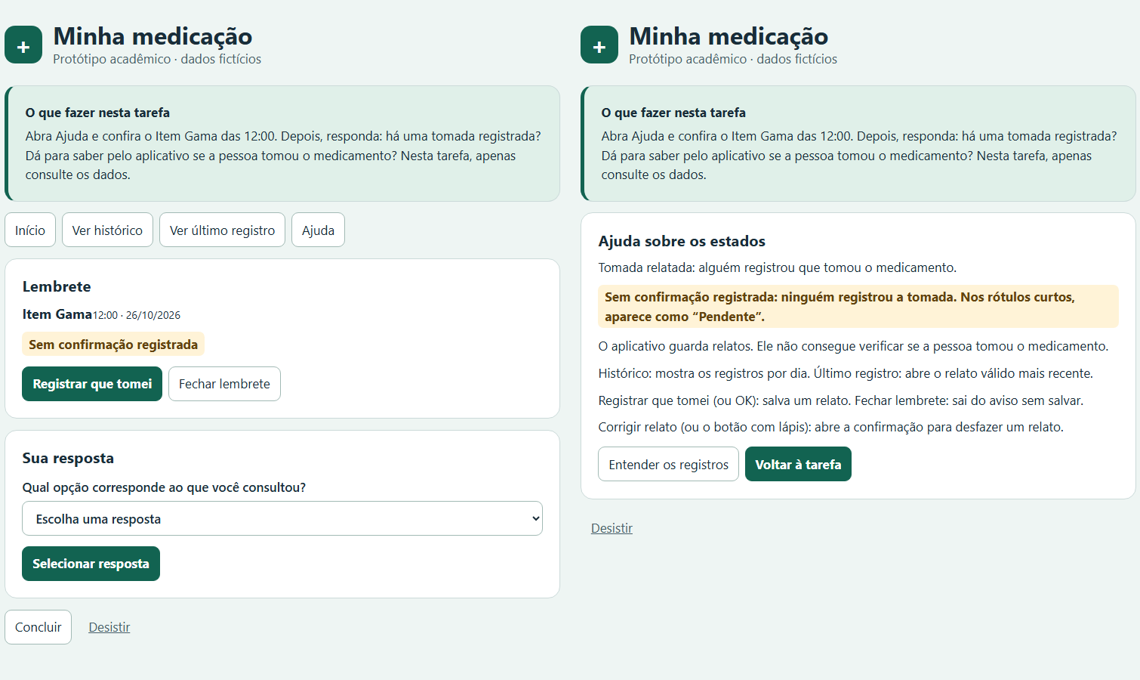
\includegraphics[width=\columnwidth]{telas.png}\\\small Lembrete e ajuda da interface 1.2. C4, variante B.\end{center}}{}

